%empezar el tp aca
\section{Diseño}

Para organizar este trabajo, lo primero que hicimos fue decidir cómo queríamos analizar el texto entrante para poder dilucidar si contenía o no malas palabras. 

Previo al diseño final estabamos casi convencidos de que el diseño debia consistir de un analizador, encargado de enviar el texto a los filtros para luego volver a recibirlo "limpio". Luego este enviaría a validar el texto enviandoselo a un objeto que tenia un criterio de aceptación para validar las palabras, fijandose si pertenecía al diccionario de palabras prohibidas para recibir finalmente el resultado que sería el que mostraba por pantalla.
A primera instancia notamos que de la forma en que estaba implementado, iba a traer resultados incorrectos ya que la ausencia de un diccionario de excepciones no permitía el ingreso de palabras válidas solo por el hecho de tener una palabra prohibida en el medio, tal como el caso de "computadora". Luego del analisis llegamos a la conclusión que este diseño, si bien cumplía con lo solicitado, se restringia a centralizar todo en el objeto organizador y esto no era realmente necesario, por lo que optamos por virar a un nuevo diseño, que es el finalmente presentado, logrando de esta forma una manera mas fácil de intercalar etapas en la cadena de proceso del texto de entrada y no tener la necesidad de modificar la construcción de la serie de filtros que se aplican.

\\
\begin{figure}[H]
\centering
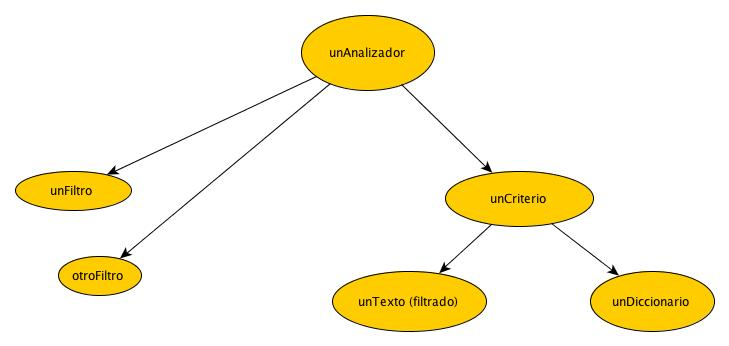
\includegraphics[scale=0.4]{../../img/disenoAnterior.jpg}
\caption{Primer diagrama de objetos sugerido: aqui se ve como el objeto unAnalizador centraliza todo el sistema }
\end{figure}
\\

Luego de debatir en el grupo, llegamos a la conclusión que el diseño de nuestra aplicación iba a constituirse por un conjunto de filtros, un diccionario de palabras prohibidas y uno de excepciones (este originalmente no estaba en los planes, pero luego nos dimos cuenta que era necesario si queríamos lograr que palabras como "computadora" no fueran detectadas como insultos).
Según nuestro diseño, al ingresarse un texto, Este llega al objeto controlador, el cual tiene una secuencia de etapas (que son nombres de clase, de las que se crear· una instancia) por las que va a ser pasado el texto. Nuestra idea es que en el controlador se configure la secuencia de filtros que se van a aplicar, el orden en que se va a hacer, y los diccionarios sobre los que se va a consultar. Por lo tanto, al definirse una secuencia de etapas, cada una de ellas va a procesar el texto de la manera que haya sido configurado para hacerlo, y luego va a enviar el texto procesado al siguiente elemento de la secuencia. Las etapas son diferentes objetos polimórficos respecto de dos mensajes, \textit{do} y \textit{prox}. En el metodo \textit{do}, cada etapa hará el proceso que le corresponda, y llamará al método \textit{prox} que está definido en la clase abstracta Etapa, que remueve el primer elemento de la secuencia, crea una nueva instancia del mismo y a ese elemento le manda el mensaje \textit{do}.

Nuestra idea es que al principio de la secuencia se definan filtros, cuya función es "limpiar" el texto para facilitar la detección de malas palabras. Por ejemplo, una de las categorías que nos comprometimos a detectar es el reemplazo de letras por sÌmbolos y/o números. Entonces, el filtro para números/símbolos define una conversión de símbolos a letras (por ejemplo, el número 5 puede representar la letra S, la @ la A, etc), y al aplicarlo al texto reemplaza esos símbolos por las letras que representan, de manera tal que al recibir el input "t@r@d0" va a convertirlo en "tarado"

Luego de aplicar todos los filtros, el texto se pasa al diccionario de excepciones, que son las que contienen una mala palabra en su interior pero que no son insultos, como computadora, con las excepciones se busca que se quiten estas excepciones del texto antes de buscar malas palabras. Una vez hecho esto, el texto está listo para ser chequeado por palabras prohibidas; en esta etapa, se define un diccionario de tÈrminos prohibidos y se busca si el texto contiene alguno de ellos, en caso de hacerlo, se vuelve al controlador con un resultado diciendo que no se aceptó el texto, y con un resultado de que sí se aceptó en caso contrario. 

Es importante remarcar que la manera que tenemos de buscar los términos prohibidos hace que soportemos algunas categorías para las cuales no hay filtros, por ejemplo, para la categoría pegado, el texto "sostarado" contiene la palabra "tarado", la cual está prohibida por lo tanto, el chequeo va a dar inválido aún cuando no se haya definido filtro para separar la palabra

Finalmente nos terminamos de convencer de optar por este diseño cuando notamos que a diferencia del diseño anterior, el diseño actual permite agregar múltiples etapas, independientemente de su tipo, es decir, sin importar si son filtros o diccionarios, teniendo como única restricción que están sean polimórficas con respecto de Etapa. Esto nos va a permitir agregar nuevas funcionalidades cuando sean requeridan sin tener que cambiar el código ya existente, permitiendo tambien así agregar nuevas categorias fácilmente

\begin{figure}[H]
\centering
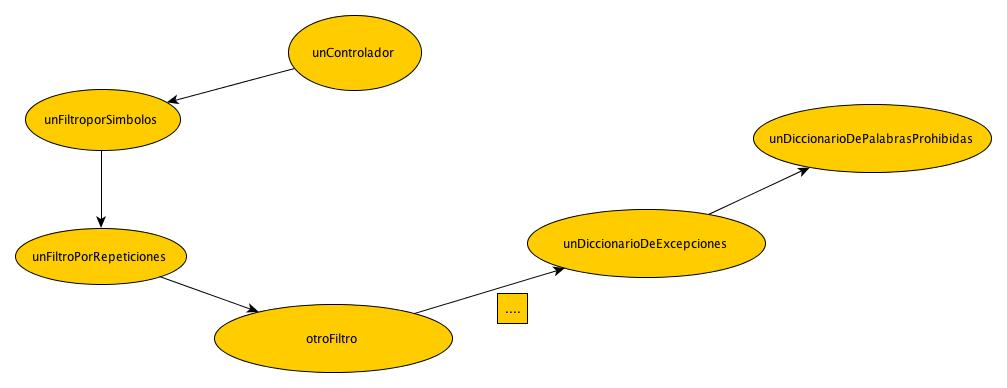
\includegraphics[scale=0.4]{../../img/disenoFinal.jpg}
\caption{Diagrama de objetos finalmente utilizado para llevar a cabo la programación del sistema}
\end{figure}

\begin{figure}[H]
\centering
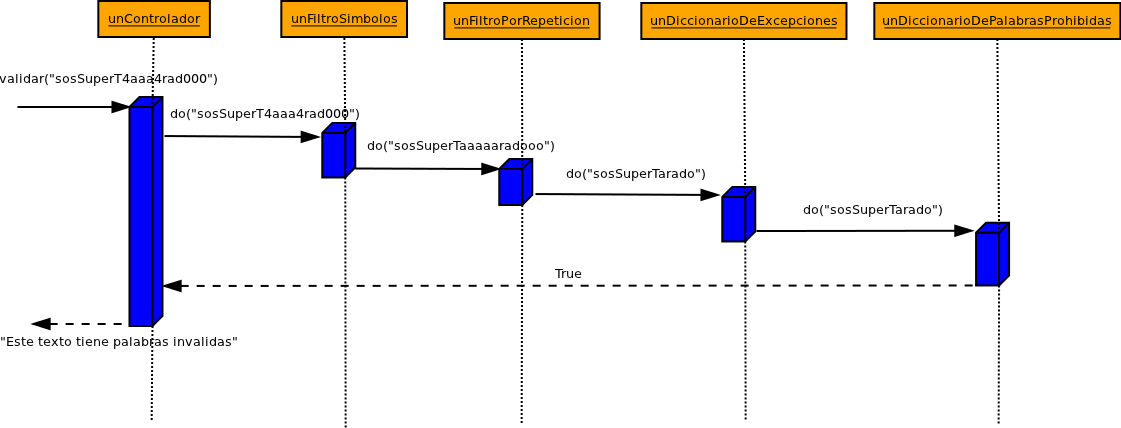
\includegraphics[scale=0.35]{../../img/sosSuperTarado.png}
\caption{Diagrama de secuencia tras ingresar el texto con insultos: sosSuperT4aaa4rad000}
\end{figure}

\begin{figure}[H]
\centering
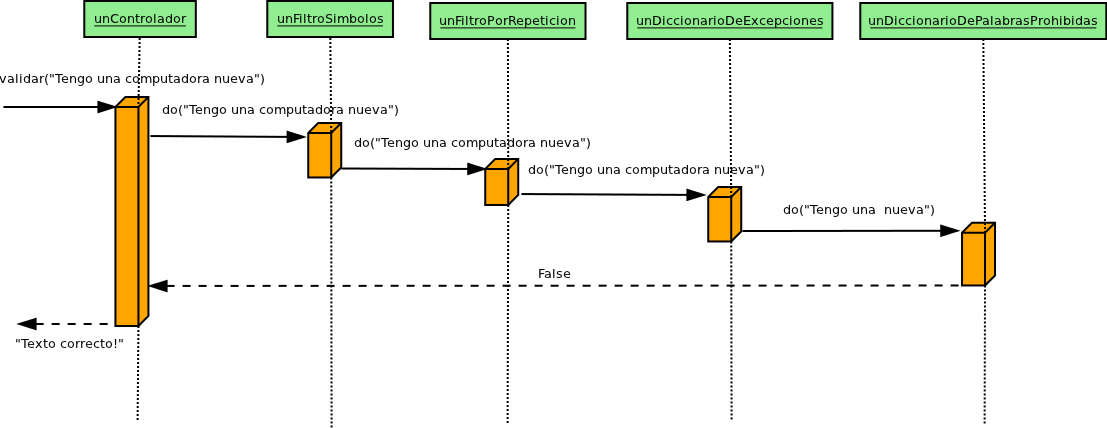
\includegraphics[scale=0.35]{../../img/computadora.png}
\caption{Diagrama de secuencia tras ingresar el texto sin insultos: Tengo una computadora nueva}
\end{figure}

\section{Retrospectiva}

Durante este sprint nos encontramos con múltiples barreras que nos llevaron a no poder cumplir estrictamente el dashboard planeado, respetando los tiempos que estimamos para el mismo.

Con el afán de obtener los mejores resultados posibles para presentar un sistema correcto, nos vimos involucrados en múltiples discusiones acerca del diseño que debiamos utilizar, que nos quitaron una gran parte del sprint ya que no lograbamos ponernos de acuerdo
Esta indecisión nos provocó un retraso importante en lo que correspondía al armado del sistema, provocando que ante la necesidad de cumplir con lo pactado no logramos llevar una correcta exhibición de las tareas que ibamos realizando en nuestro sistema de seguimiento.

En una próxima iteración creemos que deberíamos mejorar en cuanto al tiempo dedicado para tomar decisiones (Tambien demoramos mucho en poder elegir el lenguaje de programación a utilizar) y en una correcta distribución de tareas, dividiendo estas logrando explotar en mayor medidas las habilidades de cada integrante del equipo

\section{Fuente}

Rally: \href{https://rally1.rallydev.com/#/7748714472d/dashboard}{https://rally1.rallydev.com/#/7748714472d/dashboard}\\
Git: \href{https://github.com/tpsisw2/tpsisw2}{https://github.com/tpsisw2/tpsisw2}\\
App: \href{http://boiling-journey-7643.herokuapp.com}{http://boiling-journey-7643.herokuapp.com}
